\documentclass[12pt]{article}
\usepackage{../../../format}
\lhead{A Level Physics - Turning Points}

\begin{document}
\begin{center}
\underline{\huge Turning Points}
\end{center}
\section{Electrons}
\subsection{Discharge tube}
A discharge tube has a high voltage applied across it, this voltage ionises the gas. These ions then accelerate towards the cathode, hitting it with enough energy to release free electrons from the surface. These combine with the ions, emitting light.
\subsection{Thermionic emission}
When a metal is heated free electrons are released from the surface
\subsection{Determining the specific charge of an electron}
\subsubsection{Method 1}
Adjust magnetic and electric field so the flow of electrons is horizontal\\
Combine
$$eV_a=\frac{1}{2}mv^2 \ \textrm{and} \ Bev=eE$$
To get
$$\frac{e}{m}=\frac{1}{2v_a}\Bigg(\frac{E}{B}\Bigg)^2$$
\subsubsection{Method 2}
Accelerate electrons in a circle using a magnetic field perpendicular to the direction of motion.\\
Combine
$$\frac{mv^2}{R}=Bev \ \textrm{and} \ eV_a=\frac{1}{2}mv^2$$
To get
$$\frac{e}{m}=\frac{2V_a}{(BR)^2}$$
\subsection{Milikan's experiment}
\begin{figure}[h]
    \centering
    \begin{minipage}{0.45\textwidth}
        \centering
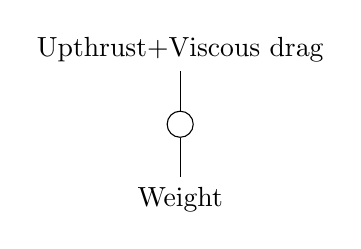
\begin{tikzpicture}[
    force/.style={>=latex,draw=black,fill=black},
    m/.style={circle,draw=black,fill=white,radius=0.3cm,thin},scale=0.5
]
    \node[m] (m) {};
    {[force,->]
        \draw (m.north) -- ++(0,1) node[above] {Upthrust+Viscous drag};
        \draw (m.south) -- ++(0,-1) node[below] {Weight};
    }
\end{tikzpicture}
        \caption{No electric field}
    \end{minipage}\hfill
    \begin{minipage}{0.45\textwidth}
        \centering
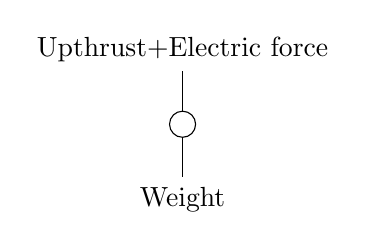
\begin{tikzpicture}[
    force/.style={>=latex,draw=black,fill=black},
    m/.style={circle,draw=black,fill=white,radius=0.3cm,thin},scale=0.5
]
    \node[m] (m) {};
    {[force,->]
        \draw (m.north) -- ++(0,1) node[above] {Upthrust+Electric force};
        \draw (m.south) -- ++(0,-1) node[below] {Weight};
    }
\end{tikzpicture}    
        \caption{Electric field}
    \end{minipage}
\end{figure}
\subsubsection{With electric field}
$$\textrm{Electric field}=\frac{QV}{d}$$
$$\textrm{Weight}=mg$$
$$\frac{QV}{d}=mg$$
\subsubsection{Without electric field}
$$F_D=6\pi r\eta v$$
$$\textrm{Weight}=mg$$
\begin{center}
Mass=Density$\times$Volume
$$\textrm{Mass}=\frac{4}{3}\pi r^3\rho$$
$$6\pi r\eta v=\frac{4}{3}\pi r^3\rho g$$
$$r^2=\frac{9\eta v}{2\rho g}$$
\end{center}
\subsubsection{Significance of results}
These results were significant because it introduced the idea of quantisation of charge
\section{Special relativity}
Special relativity is based on two postulates:
\begin{itemize}
\item The laws of physics, expressed in equations, have the same form in all inertial frames
\item The speed of light in free space is the same for all observers regardless of their state of motion and the speed of the light source
\end{itemize}
\subsection{The Michelson-Morley Experiment}
\includegraphics[width=6cm]{michelson.png}
\subsection{Relativistic momentum}
$$p=mv-\frac{m_0v}{\sqrt{1-(\frac{v}{c})^2}}$$
\subsection{Relativistic kinetic energy}
\begin{center}
Total energy=Rest energy+Relativistic KE
\end{center}
$$E_K=E-E_0$$
$$E_K=\frac{m_0c^2}{\sqrt{1-(\frac{v}{c})^2}}-m_0c^2$$
$$E_K=m_0c^2\Bigg(\bigg(1-\bigg(\frac{v}{c}\bigg)^2\bigg)^{-\frac{1}{2}}-1\Bigg)$$
Apply binomial expansion and approximation to get
$$E_K=\frac{1}{2}m_0v^2$$
\subsection{Bertozzi's Experiment}
\begin{center}
\includegraphics[width=12cm]{Bertozzi.jpg}
\end{center}
The experiment was set out to determine the variation of the kinetic energy of an electron, based on derived measurements.\\
\\
Electrons accelerated from rest, through a known P.D.\\
Gain kinetic energy = eV (Known value)\\
Calculate speed from $v=\frac{d}{t}$ (d=8.4m)\\
\\
As the bunch of electrons collided with the plate, the electrons give up their energy and the plate changes its temperature.\\
\\
Knowing the specific heat capacity and the number of electrons, the energy of one electron can be determined
$$E=\frac{mc\Delta\theta}{n}$$
\section{Wave Particle Duality}
\subsection{Electromagnetic waves}
\subsubsection{The nature of electromagnetic waves}
Electromagnetic waves are formed of perpendicular electric and magnetic fields, each of which sustain the other.\\
\subsubsection{Maxwell's Formula}
Permeability of free space - Relates the magnetic flux density of a magnetic field to the electric current that creates it\\
Permittivity of free space - Relaters the electric field strength to the charge that creates it
\subsubsection{Hertz and Radio waves}
\includegraphics[width=6cm]{hertz_1.jpg}\\
Radio waves were produced when a spark lept between the spark balls across an induction coil\\
The radio waves induce an EMF across the loop, causing a spark.\\
By placing a metal sheet in different places Hertz discovered radio waves are reflected by metal and pass straight through insulating materials.\\
By creating a standing wave and measuring the position of nodes and antinodes, the wavelength could be calculated.\\
The waves were demonstrated to be polarised when the loop was rotated 90 degrees and no sparks appeared, as the electric field was perpendicular to the loop.
\newpage
\subsubsection{Fizeau's determination of the speed of light and it's implications}
\includegraphics[width=6cm]{fizeau.jpg}\\
This experiment used a fast moving cog wheel which was increased in speed until the reflected light could not be seen. This meant that twice the distance between the wheel and the mirror would be equal to the time for a gap to be replaced by a tooth.\\
Time for one rotation:
$$T=\frac{1}{f_0}$$
Time for the wheel to move one tooth, where n is the number of teeth
$$t=\frac{T}{2N}$$
Combine the two above equations
$$t=\frac{1}{2f_0N}$$
Apply $\textrm{Speed}=\frac{\textrm{Distance}}{\textrm{Time}}$
$$c=\frac{2D}{\frac{1}{2f_0N}}=4Df_0N$$
\subsection{Microscopes}
To find the voltage required to produce electrons of a given wavelength, rearrange the equation on the formula book
$$\lambda=\frac{h}{\sqrt{2meV}}\Rightarrow \ V=\frac{h^2}{2me\lambda^2}$$
\subsubsection{Transmission electron microscope}
\includegraphics[width=8cm]{tem.png}
This involves firing a beam of electrons at a high voltage towards an ultra thin specimen.\\
When an electron wave encounters the specimen it can either:
\begin{itemize}
\item Pass straight through the specimen without interacting
\item Get absorbed
\item Diffract
\end{itemize}
The image detail can be improved by increasing the anode voltage of the electron gun.\\
Image detail may reduce when travelling through the specimen as some electrons lose speed.
\subsubsection{Scanning Tunnelling Microscope}
\includegraphics[width=6cm]{stm.png}\\
This has a very fine conducting probe very close to the surface of the sample. Quantum tunnelling means that over the very short distance there is a small probability electrons will cross the gap. A small voltage is maintained between the tip of the probe and the sample to ensure the electrons travel the right way.\\
\\
An STM can either have the probe at a constant height, and measure the current, or alter the height to keep constant current, and measure the height.
\subsection{Newton's CT of light}
Definition - Light is made up of tiny particles called corpuscles that always travel in a straight line
\subsubsection{Reflection and refraction}
Newton believed this theory was true as it can explain both reflection and refraction\\
\includegraphics[width=6cm]{reflection.png}
\includegraphics[width=6cm]{refraction.png}\\
\\
\textbf{Reflection} - These corpuscles have perfectly elastic collisions, meaning that the speed before is the speed after. The horizontal velocity doesn't change, the vertical velocity is inverted. Therefore angle of incidence equals angle of reflection.\\
\\
\textbf{Refraction} - Newton said the corpuscles were attracted into the material, causing them to travel faster, causing the component of the velocity perpendicular to the boundary to increase, causing angle with the normal to reduce. Newton was wrong.
\subsubsection{Rival theories}
Christiaan Huygens proposed the wave front theory, which is the theory we have been taught to describe refraction and diffraction. This described light travelling slower in a more dense material.\\
\\
Why Huygens' theory was rejected:
\begin{itemize}
\item It was not possible to measure the speed of light at that scale at that time, meaning neither theory could be proved correct or incorrect.
\item Newton had a better reputation
\item The wave theory only considered longitudinal waves so couldn't explain polarisation.
\end{itemize}
\subsection{The Discovery of photoelectricity}
Black body - A theoretical perfect absorber and emitter of radiation\\
Ultraviolet catastrophe - Where short wavelength radiation is incident on a black body, causing it to emit an infinite amount of power per unit wavelength
\subsubsection{The failure of classical wave theory to explain observations on photoelectricity}
\begin{itemize}
\item Wave theory suggested that given enough time, electrons would gain enough energy from a wave to escape
\item There would be a time lag between the light being incident and the emission of an electron
\item Any frequency would be able to cause electron emission given enough time
\end{itemize}
\subsubsection{Einstein's Explanation of photoelectricity}
Einstein showed electrons must have energy greater than the work function in order to escape a metal. Kinetic energy is the energy difference between the energy of the electron and the work function.
\subsection{The significance of Young's double slit experiment}
Young's double slit experiment showed interference, disproving Newton's Corpuscular Theory, however Huygen's wave theory was not accepted until Fizeau compared the speed of light in water and air.
\subsection{Wave particle duality}
By using the equations
$$\frac{1}{2}mv^2=eV \ \textrm{and} \ \lambda=\frac{h}{mv}$$
They can be used to get the equation
$$\lambda=\frac{h}{\sqrt{2meV}}$$






\end{document}